\documentclass[11pt]{amsart}
%%% WARNING: Do NOT change the page size, fonts, or margins!  Penalties will apply.


\usepackage{graphicx}
\usepackage{amssymb, amsmath, amsthm}
\usepackage{places}
\usepackage{wrapfig,floatrow}
\usepackage{varwidth, caption, subcaption} %enables \FloatBarrier, which prevents figures and tables from going below it.
%\usepackage{hyperref} %makes cross references into hyperlinks. 
\usepackage{amsmath, amssymb, amsthm, amsfonts, algpseudocode, algorithm, bbm, color, fixmath, float, graphicx, hyperref, listings, mathrsfs, mathtools, subfig, times}

%Needed commands
\newcommand*{\w}{\mathbf{w}}
\newcommand*{\x}{\mathbf{x}}
\newcommand*{\y}{\mathbf{y}}
\newcommand*{\z}{\mathbf{z}}
\newcommand*{\R}{\mathbb{R}}
\newcommand*{\E}{\mathbb{E}}
\newcommand*{\0}{\mathbf{0}}
\newcommand*{\minimizer}{\mathbf{x}^*}
\newcommand*{\dprime}{{\prime\prime}}
\newcommand{\li}[1]{\lstinline[prebreak=]!#1!}
\newcommand{\pseudoli}[1]{\lstinline[style=pseudo]!#1!}
\newcommand{\trp}{^{\mathsf T}} 
\newcommand{\im}{{i\mkern1mu}}
\newcommand{\Real}{\mathchardef\Re="023C}
\newcommand{\Imag}{\mathchardef\Im="023D}
\newcommand\norm[1]{\left\lVert#1\right\rVert}
\newcommand*\diff{\mathop{}\!\mathrm{d}}
\newcommand*\Eval[3]{\left.#1\right\rvert_{#2}^{#3}}

%Operators
\DeclareMathOperator{\argmin}{argmin}
\DeclareMathOperator{\argmax}{argmax}

%Link set up
\hypersetup{
    colorlinks=true, %set true if you want colored links
    linktoc=all,     %set to all if you want both sections and subsections linked
    linkcolor=blue,  %choose some color if you want links to stand out
    pdftitle={RL Notes},
    pdfpagemode=FullScreen
}

\endinput

%%% WARNING: Do NOT change the page size, fonts, or margins!  Penalties will apply.
%%% WARNING: Do NOT change the page size, fonts, or margins!  Penalties will apply.
% The Effect of Chemotherapy and Immunological Response on Breast Cancer Growth
\title{Breast Cancer}
\author{R. Gee, H. Fetzer, N. Suyama, J. Humpherys, O.J. Escobar}
\date{October 29 2024} % or use \today

\begin{document}
\maketitle % this actually makes the title

\begin{abstract}
Place abstract here. The abstract summarizes in one paragraph the main question and conclusions draw from your investigation.
\end{abstract}

%% First Section
\section{Background/Motivation}

Mathematical oncology is field of oncology, the study of cancer, that employs math to study cancer and its behavior.
In the words of Dr. Rockne and MD Scott, ``it [serves] as a bridge between $\ldots$ the biologist, and the practicing clinician." \cite{IntroMathOnc}
One of the biggest application of mathematical modeling in oncology is tumor growth modeling.
In mathematical oncology, tumor growth modeling seeks to understand and model the characteristics and dynamics that govern general cancer growth.
Moreover, it seeks also to understand and model the relationship between cancer and the systems that fight against it as well as the response of the cancer itself to these systems.


The primary %%%HERE deleted main (redundant
 purpose of tumor growth modeling is to first develop a general tumor growth model in the absence of any intervention.
Secondarily, it seeks to model the response to external factors such as immunological response or treatment. 
And thirdly, the modeling will then add tumor resistance and active fighting against any form of treatment be it from the immune system or other treatments.
In the absence of any intervention, several models have been made to try to show the growth of a tumor, measured by \textit{tumor burden}, denoted $T$, (see\ \ref{appendix: defs} for definitions), as a function of time $t$.
The models range from simple ODEs such as linear growth, or logistic growth, to more complicated models employing stochastic differential equations and algebraic differential equations. 
The main hope of these general growth models is to be able to use these models to develop more personable treatment to individuals facing the plight of cancer.\ \cite{YinMoes}

The more commonly used models due to their simplicity are linear, exponential, and logistic models (see Appendix\ \ref{appendix: models} for equations).
However, these do not accurately reflect the full and overall growth of observed cancers with the exception of a few cancer scenarios.
That is, they fail to generalize to the dynamics a cancer will exhibit: primarily that it has slow exponential rate and a maximal size.
In particular, the exponential model\ \eqref{eq: exp} is characterized by an infinite growth as $t$ increases which does not reflect the fact that a tumor can have a maximum size, even when considering a death rate.
Moreover, the logistic model\ \eqref{eq: logistic} converges too fast to the max size, $T_{\max}$, a tumor can be.\ \cite{Steb23}
As such, a need for a model that can firstly exhibit a slow exponential rate and then a slow convergence to the carrying capacity is preferred to others that only exhibit one of these two characteristics.

When it comes to treatment, most cancers typically use a combination for surgery, chemotherapy, and radiation therapy for treatment.
In breast cancer, surgery is the primary treatment which is not well suited for %%% HERE math->mathematical
mathematical modeling. 
Surgery removes as much as the cancer as possible so that any modeling growth would just have a sudden vertical drop in tumor burden at the time the surgery is removed causing discontinuities in the modeling.
For breast cancer, chemotherapy, be it \textit{neoadjuvent} or \textit{adjuvent} (see Appendix\ \ref{appendix: defs}), is the most common treatment supplement to surgery, being the primary treatment.

Most models for tumor growth in response to chemotherapy are primarily based on chemotherapy affecting cells at specific cell-cycles but mainly seeking to model the resistance of a specific tumor to the given drug or drugs.
Moreover, they also focus on the effects after one dose and not on a treatment plan that incorporates the frequency of the treatment.
Ophir Nave did describe that whenever chemotherapy is introduced into a model the drug would interact with both the immune system and cancer itself\ \cite{NAVE2022e09288}.
Moreover, it should also be some sort of summation of the dosage effects that wanes through the passage of time but may perhaps have a sudden and rapid change in the tumor growth as modeled by Nave in\ \eqref{eq: NavePersonalChemo}.

Most models employ a sort of %%%HERE Added of
exponential decay of the administered drug to the patient to get the rapid effect that a chemotherapy drug has on the tumor burden (e.g.\ \eqref{eq:PanettaExpDec}).
These are also specific to a certain phase of the cell state, but despite their specificity, at times ignore the negative effects on the immune system.
Further, the effect the drug has on the tumor burden is usually also attributed to only the drug itself and the effects, while at times minimal, of the immune system fighting the cancer is omitted.

%%%Changed grammar of the sentence below
Given these characteristics, it is of interest to find an expression for the effect of chemotherapy that has a rapid change in tumor burden either on all cells or at specific cell-states, as well as affecting the immune system.

The immune system naturally patrols the body in search of foreign bodies to kill and prevent diseases.
The patrolling and immediate responses are handled %%%HERE changed from given
by the innate immune system, %%%HERE Added comma
 and helper response to anything missed by the immediate response as well as targeted response is handled primarily by the adaptive immune system (see\ \ref{appendix: defs}).
This patrolling is not just for foreign bacteria but also abnormal cells such as cancer cells. 
Majority of models, like those in\ \ref{eq: dePillisTumorImmuno} or\ \ref{eq: AlharbiTumorImmuno}, look at these two parts of the immune system as  a whole and its interaction with the tumor and normal cells.
That is, they do not look at the specific immune cells interacting with the cancer other than the collective response of the immune system on tumor growth.
But as mentioned by de Pillis et. al, ``in some applications, it is not sufficient to represent the immune response with a single homogeneous population of
effector killer cells\ \cite{dePillis2014461}."
Thus, a good model, depending on the cancer, should have a more specific interaction between the immune cells that deal with that cancer in particular and the cancer itself.
If it is general, it suffices to show the interaction as whole.

The modeling for tumor-immunological response typically looks %%%HERE Added s
 at relationship between \textit{natural killer} cells (NK) and \textit{cytotoxic T}-cells (CD8$^+$) (see\ \ref{appendix: defs}) and how they affect tumor growth.
Although there are many other cells which contribute to an immune response, NK cells and CD8$^+$ cells are the only ones which directly kill the cancer cells in breast cancers\ \cite{Amens21}.
The CD8$^+$ cells are recruited to kill the cancer by the NK cells, and from this interaction arises a relation between the populations of the NK, CD8$^+$, and cancer cells. 
Unfortunately, many of the models which examine the relationship between cancer and the immune system do not include analysis of the interactions which occur once chemotherapy has begun.
Because of the immunocomprimising effects of radiation and chemotherapy, the body's ability to fight tumors naturally will decrease, leading to interesting dynamics of the cell populations.
Thus, we expect to see some description showing how the NK or CD8$^+$ cells become inhibited or die off as chemotherapy is introduced.

One important term that is used in modeling the interactions between the immune system and the tumor comes from the biochemistry equation for enzymatic reaction rates known as \textit{Michaelis-Menten kinetics}.
Specifically, the Michaelis-Menten kinetics model the rate at which an enzyme acts upon some molecule to form a complex and then act in such a way so as to produce a new product and regenerate the original enzyme.
In the context of tumor modeling, the Michaelis-Menten kinetics model the interaction between abnormal cells and the immune system, immune system and tumor cells, and tumor-tumor cell interactions.
The former describes the rate of the immune system responding to the growth of abnormal cells that could potentially become cancer.
The latter specifically considers the rate of how tumors induce other cells to become tumor cells, and the middle interaction would look at seeing specifically the rate of change between the immune system being affected by the tumor but as well as affecting the tumor itself\ \cite{math8081285}.
Hence, any model looking into the interaction of a tumor with the immune system should consider similar interactions or those modeled by Michaelis-Menten.


Given all of these characteristics for modeling tumor growth in general, as well the intricacies of chemotherapy, and then adding the difficulties of modeling immune-tumor interactions, we can gain an understanding why there is much difficulty in getting an overall general model that works for any cancer and any form of chemotherapy.
Thus, our attempt is to bring forth a model that can work in a generalized setting for a specific cancer that exhibits the known interactions and behaviors that a tumor should exhibit when facing the immune system and chemotherapy as previously outlined. 
We decided to specifically focus on breast cancer seeing that the National Cancer Institute records it as having the most number of cases as of 2024.
For the immunological response, we also focused specifically on the response given by NK and CD8$^+$ cells.
As per the chemotherapy, our focus was that of neoadjuvent therapy specific to one drug.
Lastly, our tumor growth modeling focused on a sigmoidal relationship given by the Gompertz ODE.


%% Second Section 
\section{Modeling}

%% Finite Difference methods, feel free to edit or place where you would like --Rebecca
%% In solving the original Gompertz model, finite difference methods were used because of their simplicity yet relative accuracy. The local truncation error for Forward Euler can be found as follows $\tau_i = |T^\prime(t_i) - \frac{T(t_i + h) - T(t_i)}{h}|$  where $T(t_i)$ is the actual solution at time $i$. Using Taylor Series, we can expand this to $\Bigl |T^\prime(t_i) - \frac{T(t_i) + hT^\prime(t_i) + h^2T^\dprime(t_i) + h^3T^{\prime\prime\prime}(t_i) + O(h^4) - T(t_i)}{h}\Bigr |$ which simplifies to $|-hT^\dprime(t_i) - h^2T^{\prime \prime \prime}(t_i) + O(h^3)| = O(h)$. So although quick to code and compute, there is a relatively large error term. 


%% End Finite Difference methods
\textbf{Tumor Growth}. The Gompertz model is a logistic model that was created to describe the growth of human mortality in 1825 by Benjamin Gompertz.
In particular, the ODE is given by
\begin{equation}
	\frac{\diff T}{\diff t} = k_g T \ln \biggl(\frac{T_{\max}}{T} \biggr) \label{eq: gompertz},
\end{equation}
where $k_g$ is a growth constant of the tumor, $T$ is the total number of cancer cells, and $t$ is days.
The solution to the ODE is of sigmoidal nature.
Like the logistic growth model \eqref{eq: logistic}, the Gompertz model starts off with a quasi-exponential growth at the beginning that is short lived.
However, unlike the logistic model, the Gompertz model slowly converges to the carrying capacity of the tumor population.
Figure~\ref{fig:odeModels} shows how the Gompertz model differs from that of other models used for tumor growth.

\begin{wrapfigure}[18]{R}{9cm}
  \centering
    \vspace*{-42mm}
    	\begin{varwidth}{\linewidth}
		 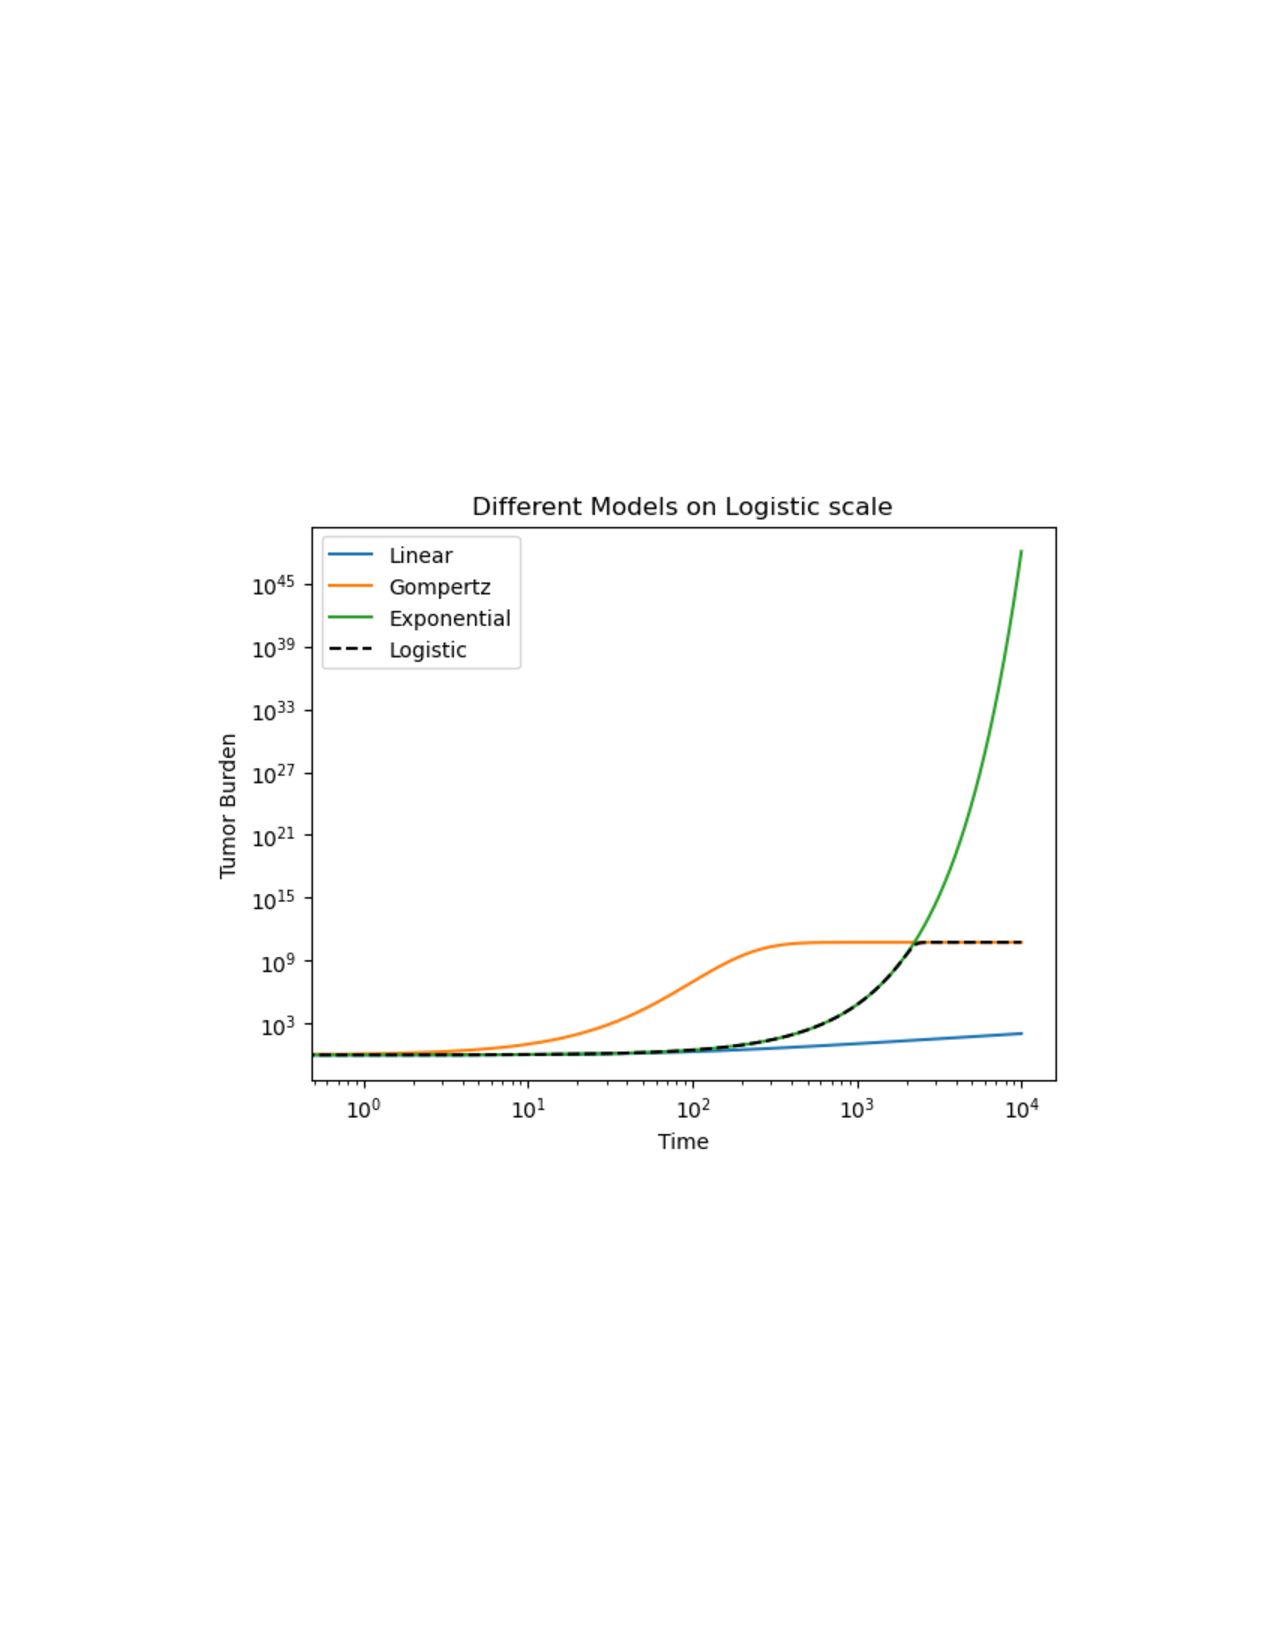
\includegraphics[scale=0.5]{./images/ode_models.pdf}
		 \captionsetup{justification=centering, width=5cm}
		 \caption{The uninhibited growth of various ODE models}
		 \label{fig:odeModels}
	\end{varwidth}
	\vspace*{-40mm}
\end{wrapfigure}

%%\begin{figure}[htb]
%%\begin{center} %Put your images in a figure like this
%%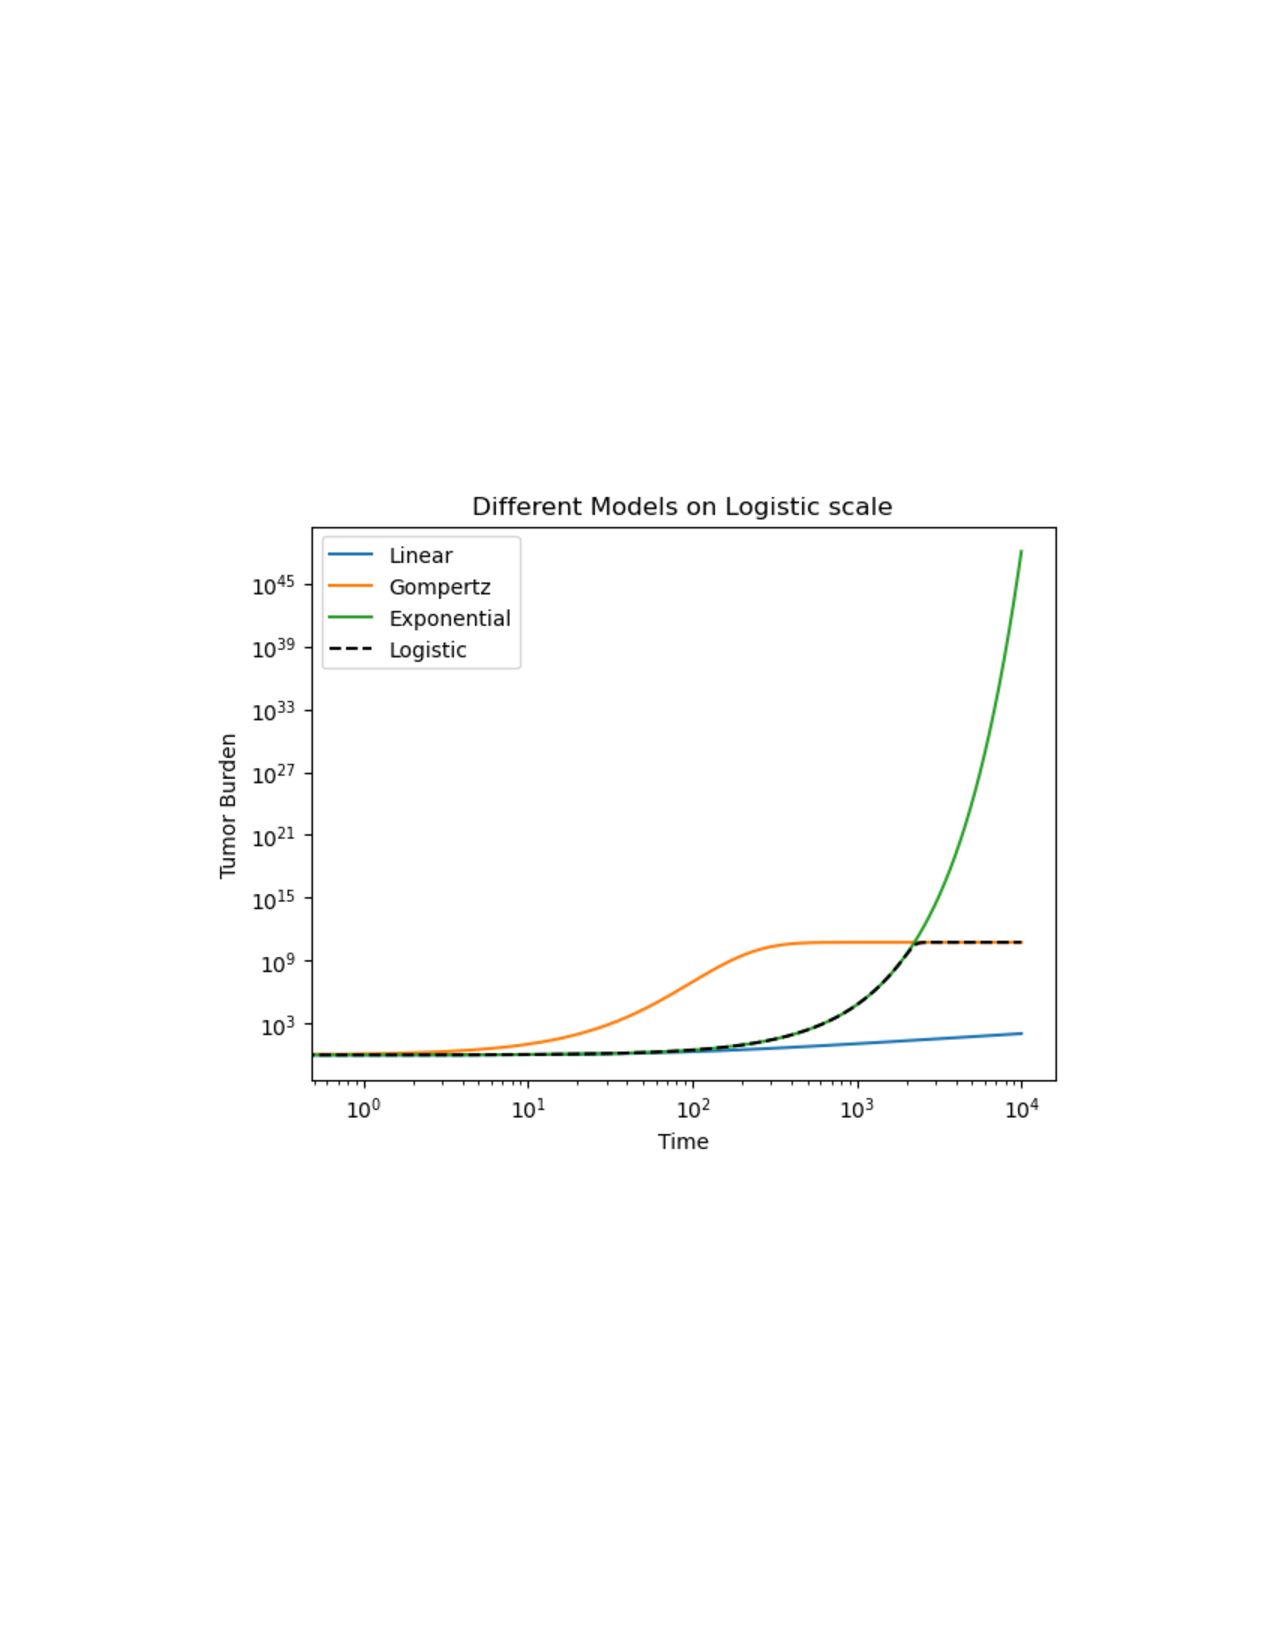
\includegraphics[width=\textwidth]{./images/logistic.pdf} 
%%\vspace*{-50mm}
%%\end{center}
%%\caption{Tumor Burden for various growth functions}
%%\label{fig:growth} % for automatic cross referencing
%%\end{figure}
Notice how the Gompertz model slows its growth earlier %%%first -> earlier
and more significantly than a logistic model while still converging towards the carrying capacity.
The logistic growth, on the other hand, is much more aggressive after its inflection point.
For the Gompertz model, take the derivative of \eqref{eq: gompertz} and set it equal to 0, this gives us that  the inflection point of the Gompertz model is at $\frac{T_{\max}}{e}$.
This is the point when 36.8\% of the carrying capacity has been reached compared to the inflection point of the logistic model that occurs at half the carrying capacity.
As stated earlier, we wanted a model that exhibits an exponential growth but also has a slow convergence to the carrying capacity.
This is why the Gompertz is a better modeling choice than other given models\ \cite{LairdGompertz}. 

\textbf{Chemotherapy}. For chemotherapy effects, seeing that models are derived as exponential decays of the drug-dose and are dependent on the type of drug administered as well as the percentage of cancer killed at a specific cell-state, we opted to work with the model proposed by Bethge et al (which is similar to the one given by de Pillis and Radunskaya\ \eqref{eq: Pillis}). The chemotherapy differential expression is
\begin{equation}
	f \mu c(t) T, c(t) = e^{-\gamma t} \label{eq: chemo},
\end{equation}
where $\mu$ represents the drug sensitivity of cells (thereby implying drug effectiveness), $c(t)$ is the concentration of the given drug with a rate modeled by a decay constant $\gamma=\frac{\ln{2}}{t_{1/2}}$ after the half-life of the drug, and $f$ is %%%Deleted extra "is"
the proportion of cells that are in specific cell-cycle such that chemotherapy affects those cells specifically.
If the given drug affects all cells equally irrespective of cell cycle, then $f$ is equal to 1.

The chemotherapy differential expression specifically models the rate of change, with respect to time, of the death or removal of tumor cells by the given drug.
At $t=0$, we would expect a high number of cells to be killed off, and as time continues, we would expect to see that the effectiveness of the drug decaying off and thereby the proportion of tumor cells killed also decreases.
Moreover, depending on how good or strong the drug is, we would expect to have a different rate of change which is the purpose of the half life in $\gamma$ and the $f$ constant.
Adding \eqref{eq: chemo} to our growth in \eqref{eq: gompertz} gives 
\begin{equation}
	\frac{\diff T}{\diff t} = k_g T \ln \biggl(\frac{T_{\max}}{T} \biggr) - f \mu c(t) =k_g T \ln \biggl(\frac{T_{\max}}{T} \biggr) - f \mu e^{-\gamma t} \label{eq: gompertz-chemo}.
\end{equation}

\textbf{Immune}. Having now considered chemotherapy, we opted to also include the influence of the immune system on the tumor burden of a patient. The basis of our immune system modeling comes from an already published model which focuses on the interaction between cancer cells, NK cells, and CD8$^+$ T-cells \cite{Immune}. While there are many more cells that influence tumor burden, these are the two cells that act directly on breast cancer cells \cite{Amens21}. In the following differential equations, T is the tumor cell population, N is the NK cell population, and L is the CD8$^+$ T-cells population. The changes of these populations are modeled as

\begin{equation} 
	\frac{\diff T}{\diff t} = aT(1-bT) - N_{KR}NT - D \label{eq:dT}
\end{equation}
\begin{equation} \label{eq:dN}
	\frac{\diff N}{\diff t} = \sigma - N_dN +\frac{gT^2}{h + T^2}N - pNT
\end{equation}
\begin{equation} \label{eq:dL}
	\frac{\diff L}{\diff t} = - mL +\frac{jD^2}{L_R + D^2}L - qLT + rNT
\end{equation}
\begin{equation} \label{eq: D}
	D = d\frac{(L/T)^\lambda}{s + (L/T)^\lambda}T
\end{equation}

Due to the complexity and number of constants, we define and quantify them in Appendix\ \ref{appendix: models}, but we will break down the system of immune ODEs. 
In equation\ \eqref{eq:dT}, the tumor cell population increases by a single component, $aT(1-b)$, which is the logistic growth  of the tumor. The remaining two terms $N_{KR}NT$ and $D$ signify the proportion of tumor cells killed by NK cells and CD8$^+$ cells, respectively.
In equation\ \eqref{eq:dN}, the NK cell population increases due to two components. One is the constant inflow of cells independent from tumor influence, denoted $\sigma$, and the other is the increase of NK cells due to the tumor's presence. This term takes the form of a Michaelis-Menten kinetics equation, and is denoted $\frac{gT^2}{h + T^2}N$. The remaining two terms of this equation are decreases in NK cell population. The first being natural NK cell death, denoted $N_dN$, and the last one being the proportion of NK cells deactivated by tumor cells, denoted $pNT$.

For equation\ \eqref{eq:dL}, we again have two components which are loses in CD8$^+$ T-cells population, the terms $mL$ and $qLT$. The first component is the proportion of naturally dying cells, and the second is the proportion deactivated by tumor cells. We also find two components contributing to an increase in CD8$^+$ T-cells, the first being $\frac{jD^2}{k + D^2}L$, the proportion of CD8$^+$ cells recruited to fight cancer, again in the form of a Michaelis-Menten kinetics equation. Lastly, the term $rNT$ models the phenomenon where CD8$^+$ cells are produced after an NK cell is killed by a tumor cell. 


\textbf{Unified Model}. The combination of the three models requires some thought.
The Gompertz-Chemo integrated model for tumor burden can be added in place of the logistic growth factor in the immune system model, but the effects of the chemotherapy on the immune cells cannot be ignored.
Although sources were inconclusive on whether the chemotherapy directly killed the NK and CD8$^+$ cells, it is known that all cells are negatively affected by the therapy, mainly being inhibited in their ability to kill cancerous cells\ \cite{RebeCytoChemonImmune}.
We make the assumption that the number of NK and CD8$^+$ cells affected by the chemotherapy is proportional to\ \eqref{eq: chemo} and the number of NK and CD8$^+$ cells. 
As such, we introduced a term in the differential equations for both CD8$^+$ cells and NK cells that seeks to replicate the natural inhibition CD8$^+$ and NK cells experience.
Specifically, the term ``kills"\footnote{We thought of this with an analogy 20 workers where only 5 are actively working, so that 15 workers are ``dead" at work. While this is a very naïve assumption, it does help exhibit inhibition.} in proportion to their interactions with the chemotherapy drug.

Moreover, in their Chemotherapy for Breast Cancer page, the American Cancer Society states that typically chemotherapy will be around 3-6 months which gives about 8-12 \textit{treatment cycles} (see\ \ref{appendix: defs}).
Hence to properly show inhibition, we altered the parameter at the end of \eqref{eq: NK} and \eqref{eq: CD8} until simulations predicted at least 5 rounds of chemotherapy before \textit{remittance} (see\ \ref{appendix: defs}).
This results in the following system of equations.

\begin{equation} \label{eq:unifiedmodel}
\frac{\diff T(t)}{\diff t} = k_g T(t) \ln \biggl(\frac{T_{\max}}{T(t)} \biggr) - f \mu e^{-\gamma t} - n_{kr}N(t)T(t) - D 
\end{equation}
\begin{equation} \label{eq: NK}
\frac{\diff N(t)}{\diff t} = \sigma - n_dN(t) +\frac{g(T(t))^2}{h + T^2}N - pN(t)T(t) - N(t)f \mu e^{-\gamma t}
\end{equation}
\begin{equation} \label{eq: CD8}
\frac{\diff L(t)}{\diff t} = - mL(t) +\frac{jD^2}{l_r + D^2}L(t) - qL(t)T(t) + rN(t)T(t) - Lf \mu e^{-\gamma t}
\end{equation}
\begin{equation} \label{eq:Dconst}
D = d\frac{\Bigl(\frac{L(t)}{T(t)}\Bigr)^\lambda}{s + \Bigl(\frac{L(t)}{T(t)}\Bigr)^\lambda}T(t)
\end{equation}
The constants and form of the equation should be familiar, as they are taken directly from the above equations. 

To begin modeling, we called $t_o=t=0$ to be the time when a tumor should be of sufficient size that a person, medical practice, or immune system should be able to identify or detect the cancer.
While it is unknown why cancer can go undetected completely from the immune system or medicine, there are estimates for a tumor burden that should be detectable. 
Specifically, Caley and Jones state that when cancer is detectable there are about $10^8$ to $10^9$ tumor cells in the body\ \cite{CALEY2012186}. 
Since it was part of our interest to examine whether our model would show a tumor growing to its $T_{\max}$ without much immunological intervention, we began with an initial tumor burden of $T_o = 9\times10^8$ (number of cells) as shown in Figure~\ref{fig:FullODE}.
Moreover, we assumed a doubling in size every 180 days.
As per the chemotherapy, we opted to start the treatment at $45$ days from $t_o$ to account for the time a patient has between waiting for biopsy results, further lab tests, and the actual start of the chemotherapy.

\begin{figure}[h!]
\vspace*{-3mm}
\begin{center} %Put your images in a figure like this
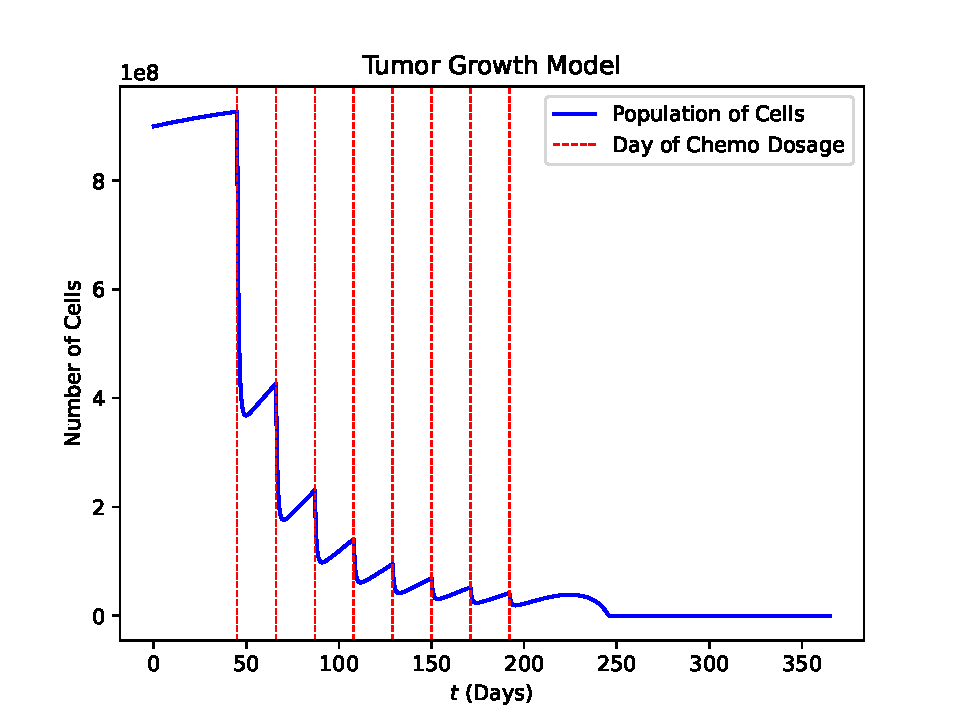
\includegraphics[scale=0.6]{./images/growth_8T_3W_C45.pdf} % Better to make them pdfs than png or gif or jpeg
\end{center}
\caption{The growth of breast cancer  as modeled by \eqref{eq:unifiedmodel} for 8 cycles with each one occurring every 3 weeks for $T_o=9\times 10^8, T_{\max}=9\times10^9$.}
\label{fig:FullODE} % for automatic cross referencing
\end{figure}

One of the harder aspects was to control the initial population of NK and CD8$^+$ cells.
However, we used the ratio of NK cells to mm$^2$ of tumor area given by Larsen et al to calculate a starting number of local NK cells.
In particular, the ratio we used was that of 1 NK cell per 50mm$^2$ of tumor tissue area since their paper proposes that 1:35 is an ``at-best" estimate for high-NK-density tumor tissue\ \cite{SopikTumorSize}.
As for the immune cells, while the ratio of NK cells to CD8$^+$ is unknown, it is known that, overall, CD8$^+$ cells make up a larger immune cell count than NK, so we assumed
a ratio of 4 CD8$^+$ cells per 1 NK cell.
To then compute the starting number of immune cells, we used geometry to calculate the area of $T_o$ assuming each breast cancer cell has an average diameter size of 15 $\mu$m\ \cite{BabitaShashni2018b17-00776}.

Having initial conditions, to solve the system of ODEs in\ \eqref{eq:unifiedmodel} -  \eqref{eq:Dconst}, we used \begin{verbatim} scipy.integrate.solve_ivp \end{verbatim}
that uses the explicit Runge-Kutta method of order 5(4).
That is, we used an embedded Runge-Kutta method where a 5$^\text{th}$ order method approximates the solution and a 4$^\text{th}$ order method is used to estimate the local truncation error.
This allows for effective error estimation and enables an adaptive step size control\ \cite{DORMAND198019}.
Our results are displayed in Figure~\ref{fig:FullODE}.
As we solved for the tumor burden, we also solved for the immune cell counts.
These are given in Figure~\ref{fig:NKCD8_log_growth}.

\begin{figure}[h!]
\centering
	\begin{subfigure}{.5\textwidth}
  		\centering
 		 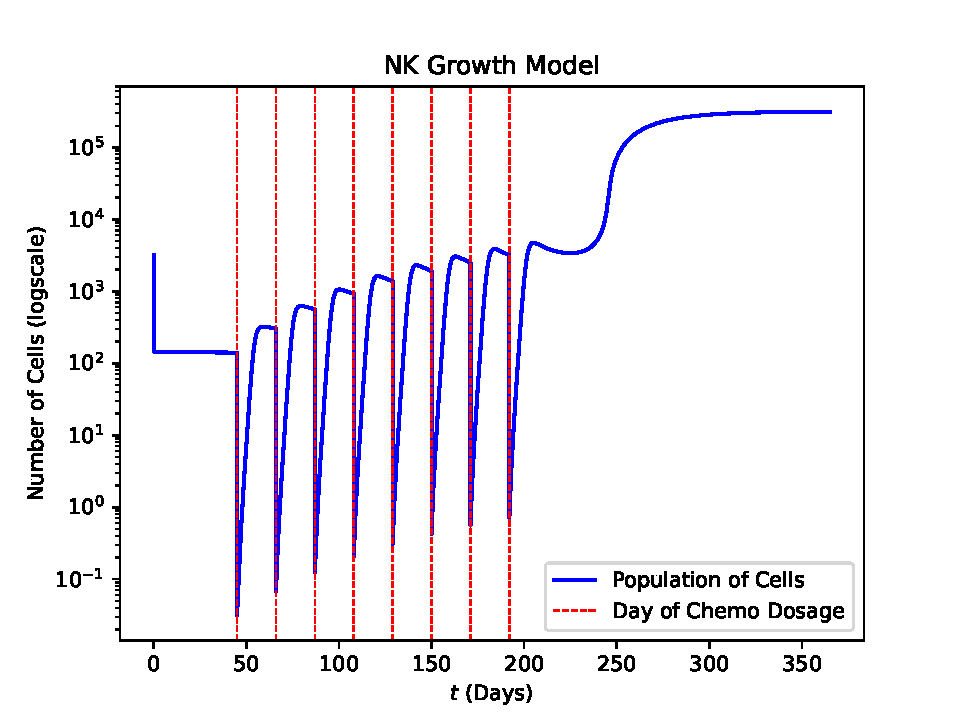
\includegraphics[scale=0.43]{./images/NK_growth_8T_3W_C45_semiy.pdf}
 		 \caption{NK growth starting at $\log(3.2\times 10^3)$.}\label{fig:NKGrowth}
	\end{subfigure}%
	\begin{subfigure}{.5\textwidth}
  		\centering
  		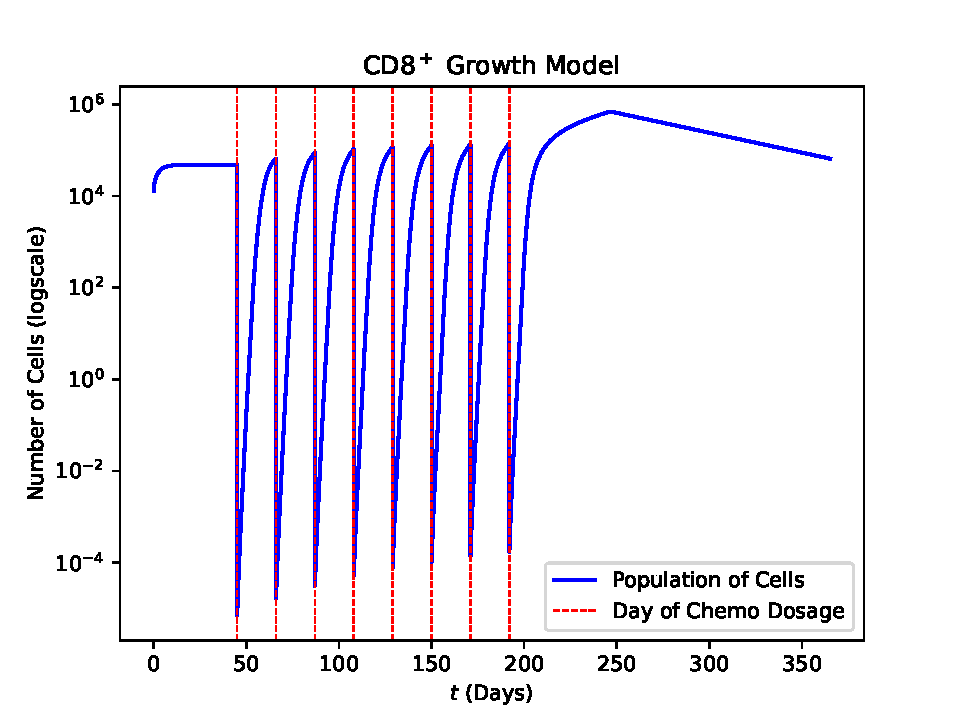
\includegraphics[scale=0.43]{./images/CD8_growth_8T_3W_C45_semiy.pdf}
  		\caption{CD8$^+$ growth starting at $\log(1.3\times 10^4)$.}\label{fig:CD8Growth}
	\end{subfigure}
	\caption{The growth of immune cells in relation to the tumor of Fig~\ref{fig:FullODE} as given by \eqref{eq: NK} - \eqref{eq:Dconst}.}\label{fig:NKCD8_log_growth}
\end{figure}

The easier parts to model were chemotherapy treatments as those only needed a summation of \eqref{eq: chemo} for however many terms we needed.
This reflects the amount of chemotherapy drug in the body after multiple doses.
Moreover, the model also shows a constant proportion of tumor cells killed by the drug as stated in\ \cite{CALEY2012186}.
The harder aspects, as mentioned earlier, were the initial conditions that could well represent what happens naturally in the body as well as possible tumor capacities and the inhibition immune cells experience. 

For some abnormally large but medically recorded tumor burdens that we assumed to be our tumor capacity, our model predicts steep exponential growth.
That is, we assumed that recorded tumors of size 91$mm$ and on, having at least a 60\% probability of killing an individual\ \cite{SopikTumorSize}, were the carrying capacity for breast cancer.
With the lower bound of 91$mm$, our model would grow very quickly, never tapering off, and once chemotherapy started, the tumor burden would decrease (see Figure~\ref{fig:abnormal_growth} in Appendix \ref{appendix:graphs} for an example) as expected.
However, once the chemotherapy sessions were done, the growth is exponential and rather quick.
Even the most aggressive tumors do not double in under 100 days.
Thus, our attempt to model any possible tumor growth capacity under any starting initial condition was a failure.

Our initial approach was also to begin modeling at the moment one cancer cell appears in the body (see\ \ref{fig:1cellgrowth} in\ \ref{appendix:graphs} for an example).
However, given our modeling and constants, the tumor was unable to survive for longer than about 10-15 days.
The main factor in the dying of the tumor was the immune system intervening with the cancer rather quickly.
This of course does not happen with everyone as unfortunately there are people who develop cancer.
This is what led us to changing our approach of looking at the dynamics at a point where the tumor is of significant size that the immune system cannot kill off the cancer on its own, which is our designated $T_o$.
%%% Potentially talk about how we also aimed at starting at 10e8 but that did not work as the immune system killed off a good chunk before chemo even started.

%%% In the paper of Sopik and Narod, they estimated the probability of dying from breast cancer as a function of the size of the tumor and found that, while some primary tumor sizes can be as big as 150$mm$ in diameter, the mortality probability plateaus starting with tumors with a diameter of  91$mm$\ \cite{SopikTumorSize}.
%%% Specifically, the mortality probability of tumors with a  diameter of 150$mm$ is about $64.1\%$ whereas tumors with a diameter of size ranging from $91-100 mm$ exhibited a $60\%$ mortality probability.
%%% Thus, there is not much of an increase in chance of death with a bigger tumor size.
%%% Hence, our $T_{\max}$ became the number of cells found in a tumor of $mm$ in diameter.
%%% Larsen et al found that, on average and in a highly dense colorectal carcinoma, there is about 35$mm^2$  of tumor tissue\ \cite{LarsenStineNkCellsRatio}.


%% Third Section
\section{Results}
%Here we have a forward Euler numerical method approximating the tumor burden with and without a single session of chemotherapy. 
%We see that without chemotherapy the cancer grows exponentially. 
%On the other hand, after a session of chemo, 
%we see a sharp decline followed by a continuation of exponential growth

%%\begin{figure}[h!]
%%\begin{center} %Put your images in a figure like this
%%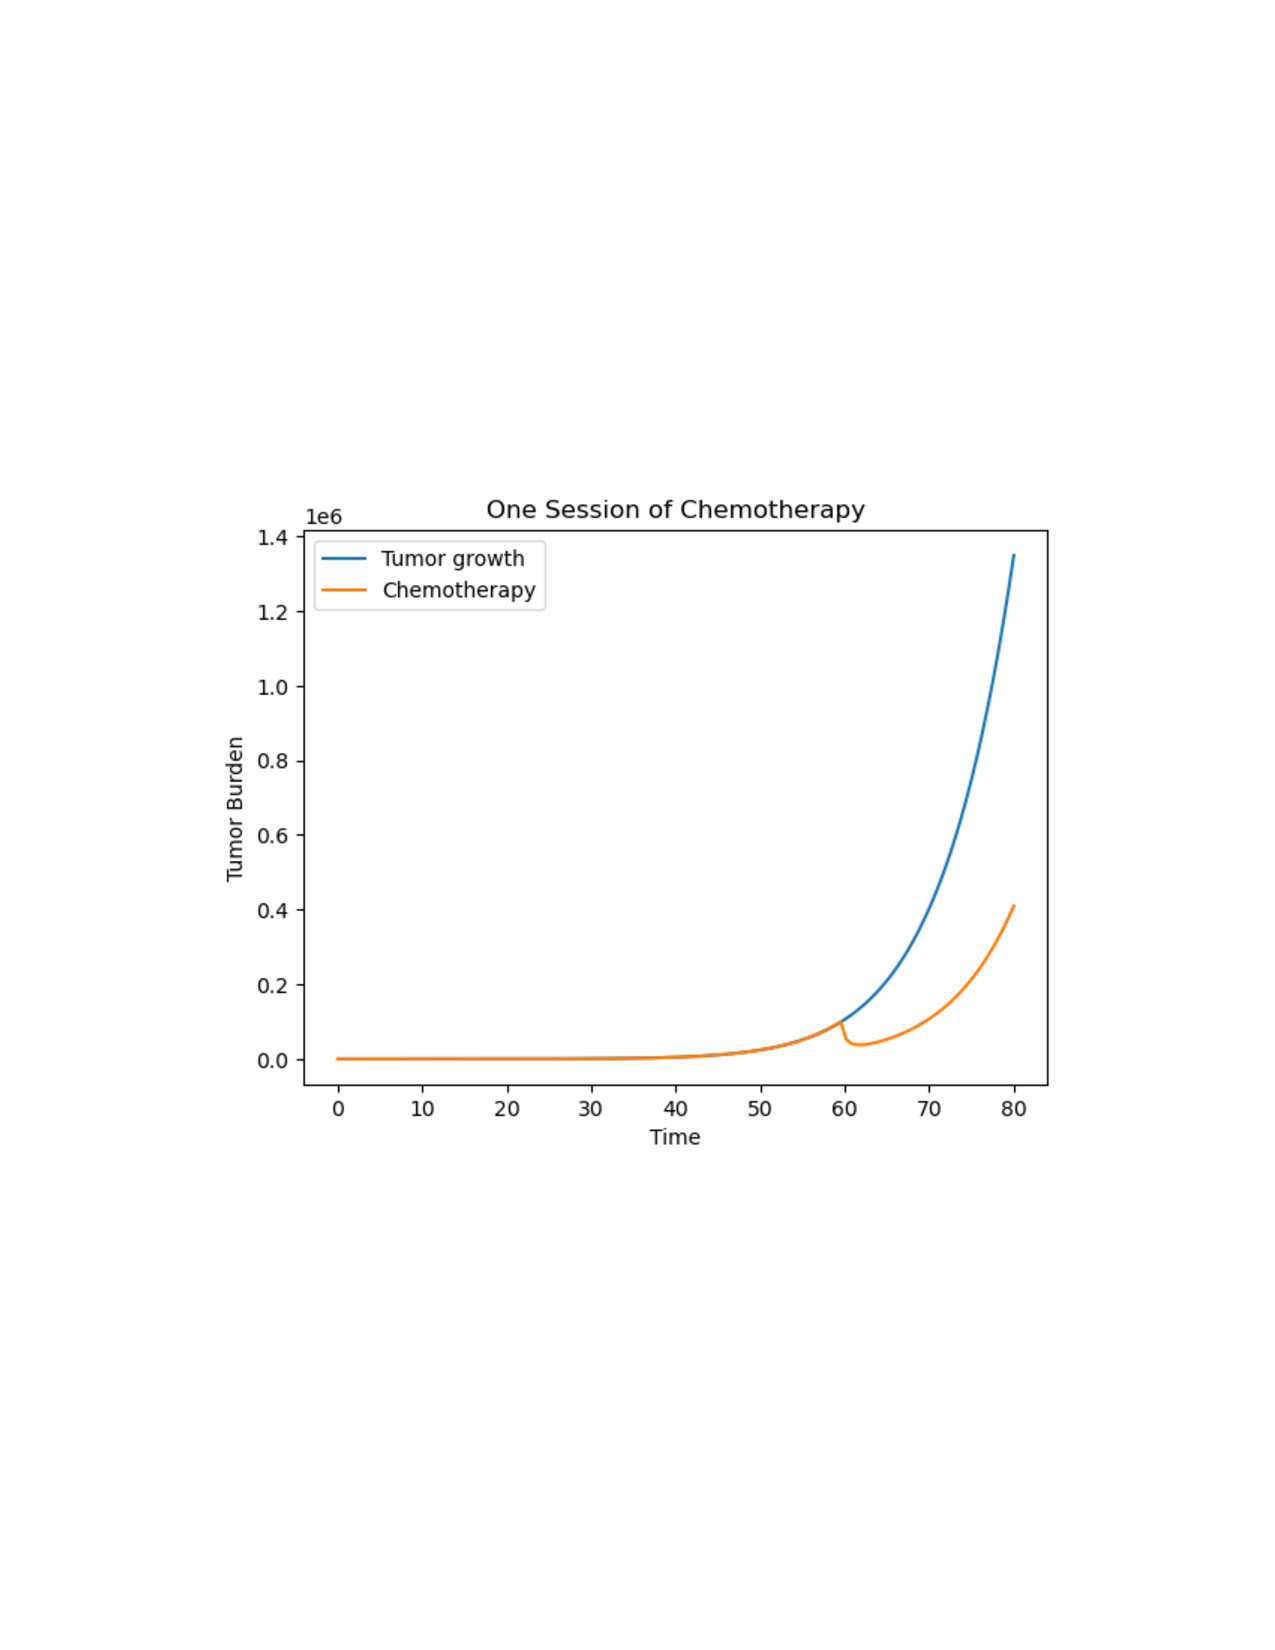
\includegraphics[width=\textwidth]{./images/chemo.pdf} 
%%\vspace*{-50mm}
%%\end{center}
%%\caption{Tumor burden with vs without chemo session}
%%\label{fig:chemo} % for automatic cross referencing
%%\end{figure}

As mentioned earlier, starting at $(t_o, T_o)$, we can see in Figure~\ref{fig:FullODE} that our model exhibits growth for an amount that should, in theory, not yet be detectable.
 Our model initially does well in describing the dynamics that tumor burden should exhibit on the premise the immune system has not yet fully detected it.
That is, our model exhibits a tumor that remains ``undetectable" to the point that it grows seemingly without bound.
For any interactions with local NK cells, these are relatively low so that overall trend of the tumor burden is that of growth and there is not much recruitment of CD8$^+$ cells.

Another important aspect of our model as displayed in Figure~\ref{fig:FullODE} is the successful modeling of the remission of cancer.
Though hard to gauge due to the scale of our image (see Figure~\ref{fig:FullODE_semiy} in \ref{appendix:graphs} for a log-scale version), we can see the cancer levels reach values that are near zero.
This seems to connect well with the aforementioned cycle length of 3-6 months.
Moreover, when we look at the cell count for NK and CD8$^+$ cells, as shown in Figure~\ref{fig:NKCD8_log_growth}, we get can conclude that the neighboring patrolling NK cells fight the cancer and die off which results in a spike of CD8$^+$ cells.
This again connects with what we know happens in real life wherein CD8$^+$ cells must get recruited and trained to kill cancer but only after the initial NK cells do the first response.
Thus, our overall system of ODEs does well in 


Despite our good results, our model did suffer from various weaknesses.
One of the bigger weaknesses is that for bigger tumor burden capacities, that have been recorded, our model would predict very rapid exponential growth (see Figure~\ref{fig:abnormal_growth}).

The fully integrated cancer model with both chemotherapy and immune cells predicts unreasonable results for chemotherapy without additional adjustments. For reasonable initial tumor sizes, one or two rounds of chemotherapy almost immediately kill the tumor. In practice, patients undergo 5-8 rounds of chemotherapy on average before showing signs of remission. Such problematic behavior is likely a result of the immune model, which as presented in a previous paper does not generalize well past 30 days. Thus, we tweaked our initial full model to produce qualitatively sound results.


%%Fourth Section
\section{Analysis/Conclusions}

First, in analyzing our model, we use known mathematical methods to analyze its stability as an operator.
The system is not linear, so we cannot simply take the eigenvalues of the operator. 
We try to analyze the system by linearizing around the equilibrium solution. 
The equilibrium solution that makes the most sense is where there are no cancer cells or CD8$^+$ cells and a steady number of natural killer cells. 
This corresponds to $T=0, L=0, N=\sigma/(N_d)$.   

Some nuance is necessary as there are zeros in the denominators at this point, but a simple mathematical analysis shows that the limits do exist. 
We take the Jacobian of the system of equations to linearize\ \eqref{eq:JacobianBastard}. 

Note that this cannot be evaluated at our equilibrium solution as $\left(\frac{T_{\max}}{T}\right)$ is not bounded as $T \rightarrow 0$. 
The linearization of the model fails to exist at the equilibrium, and thus we would expect the model to be very sensitive and unstable.

Overall, our model still demonstrates that ODEs are a promising way to model breast cancer growth. 
The predicted effect specifically of chemotherapy is appealing. 
However, initial conditions strongly affect our model.
Both our stability analysis and graphs show that slight changes in initial conditions drastically alter results qualitatively.

When we examine the parts of our model, the most promising is the model of chemotherapy alone. 
Our model predicts, as expected, that a single round of chemotherapy strongly weakens a tumor in the first few days before the tumor rebounds. 
Without the immune response, though, no number of chemotherapy treatments protects against the tumor growing exponentially after the last treatment.

In our full model, the immune system successfully kills cancer after the last treatment, but the immune system component of the model remains a weak point. 
The immune system model on its own performs poorly in the long term.
It experiences discontinuities and negative cell populations after only 30 days (see Figure~\ref{fig:forward}).
Initial conditions also highly affect the results of the immune model.
When we integrate the immune system into our full model, we mitigate a lot of negative consequences by inhibiting immune cells with chemotherapy.
However, our immune system equations still contribute to our model's sensitivity to initial conditions.

Another weakness of our model is the uncertainty of our parameters.
Most of these parameters were found experimentally, but with different experiments under varying assumptions.
Moreover, when we introduced a parameter to our final model to inhibit immune response due to chemotherapy, we simply chose a value which produced convincing qualitative results.
Fully inspecting and adjusting our parameters would be difficult, but would make our model more quantitatively correct.

Several simplifying assumptions also weaken our model. 
Primarily, we do not incorporate tumor resistance to chemotherapy drugs, which is know to occur in almost all forms of cancer.
Secondly, unlike other attempts to model tumor burden, we did not consider normal cells in the area with cancer.
Including normal cells could drastically affect the dynamics of our model because the immune system would split between fighting cancerous normal cells as well as the tumor.
Additionally, we modeled chemotherapy with a single drug that affects all cancer cells.
Typically, chemotherapy involves several drugs which affect cancer cells in different stages.
Finally, our full model includes a term which indicates that chemotherapy kills immune cells.
Purportedly, chemotherapy only inhibits immune cells, but since we model immune cell population, that information is hard to incorporate.

If our model accurately predicted tumor burden, it might be useful to monitor the affect of treatment cycles and doses of one prescribed drug on breast cancer patients. 
Given previous measurements of tumor burden and immune cells, doctors could predict when a patient will be in remission and corroborate the patient's remission status with the tumor growth model. 
Given more time, we might further inspect whether the model accurately predicts outcomes given insufficient treatment, alter our parameters, or reexamine any of our simplifying assumptions.

\newpage

\appendix

%%%%%%%%%%%%%%%%%%%%% Graphs %%%%%%%%%%%%%%%%%%%%%%
\section{Supplemental Graphs}
\label{appendix:graphs}
In this section, we give more graphs that help our analysis as supplementary information to the main points and graphs given in the paper.
\begin{figure}[H]
\vspace{-2mm}
\begin{center} %Put your images in a figure like this
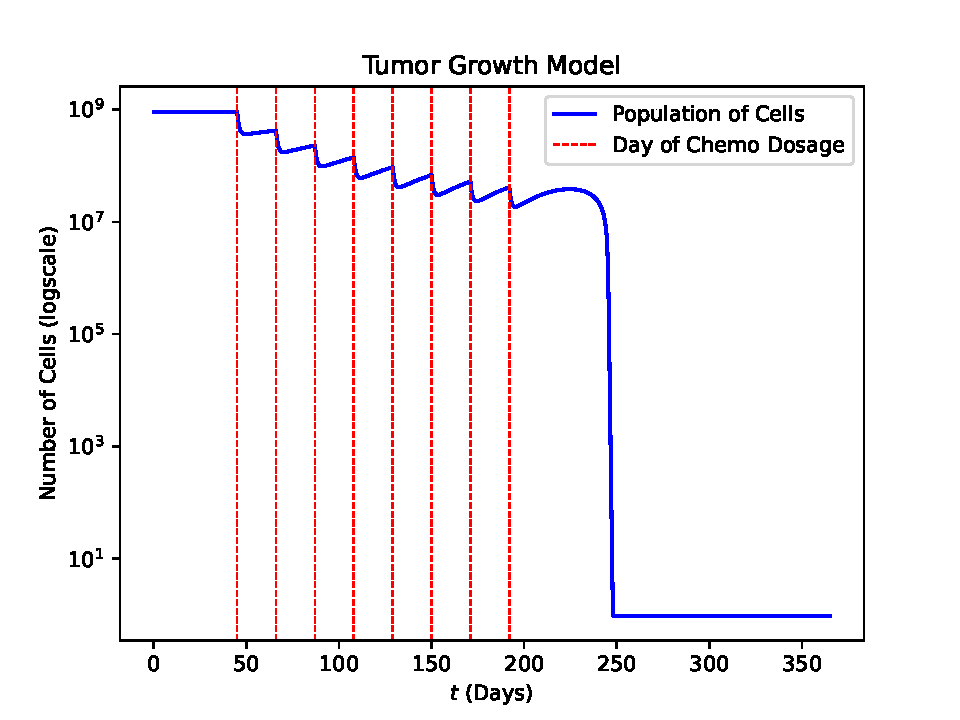
\includegraphics[scale=0.6]{./images/growth_8T_3W_C45_semiy.pdf} % Better to make them pdfs than png or gif or jpeg
\end{center}
\caption{The growth of breast cancer, in a semilog scale for $T$, as modeled by \eqref{eq:unifiedmodel}. Compare to Figure~\ref{fig:FullODE}. This graph helps us appreciate the actual death of cancer to near zero.}\label{fig:FullODE_semiy} % for automatic cross referencing
\end{figure}

\begin{figure}[H]
\begin{center} %Put your images in a figure like this
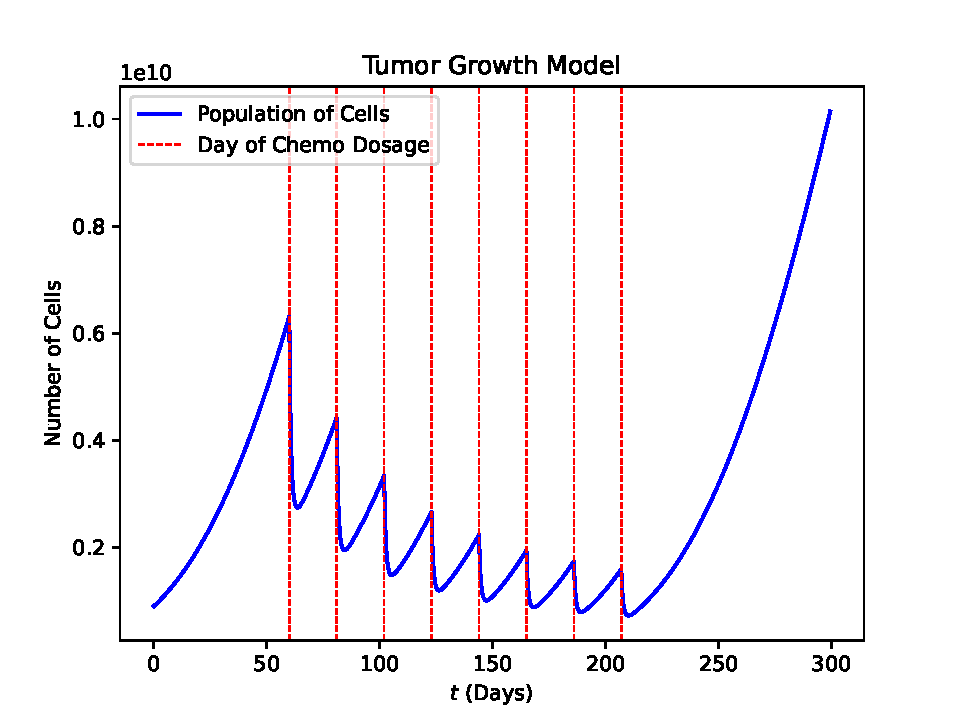
\includegraphics[scale=0.6]{./images/abnormal_growth_8T_3W.pdf} % Better to make them pdfs than png or gif or jpeg
\end{center}
\caption{Growth given by an abnormally big tumor capacity of size at least $91$mm in diameter.}\label{fig:abnormal_growth} % for automatic cross referencing
\end{figure}

\begin{figure}[H]
\begin{center} %Put your images in a figure like this
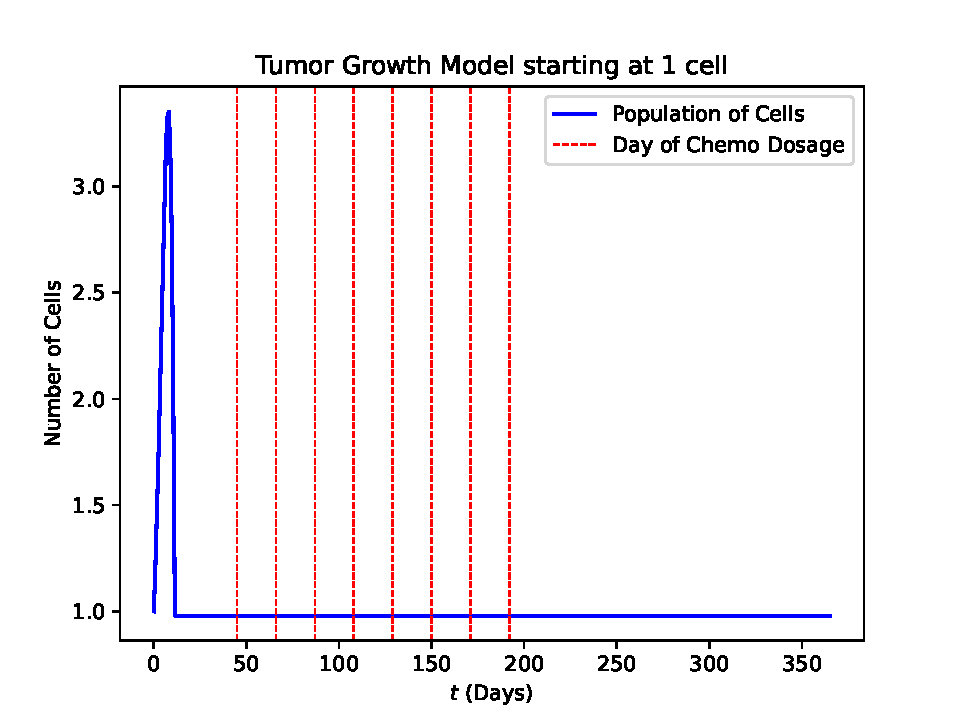
\includegraphics[scale=0.6]{./images/growth_1cell.pdf} % Better to make them pdfs than png or gif or jpeg
\end{center}
\caption{Tumor growth starting from 1 cell.}\label{fig:1cellgrowth} % for automatic cross referencing
\end{figure}

Here we plot the differential equations of the immune system. 
We get our initial values from a plot in the paper where we got the differential equations. 
In the paper published, the populations only go to about 35 days. 
Below we've created similar plots, but as we increase the time beyond 35 days, 
we start to see some problems, which we will address in the analysis/conclusions section.

\begin{figure}[H]
\begin{center} %Put your images in a figure like this
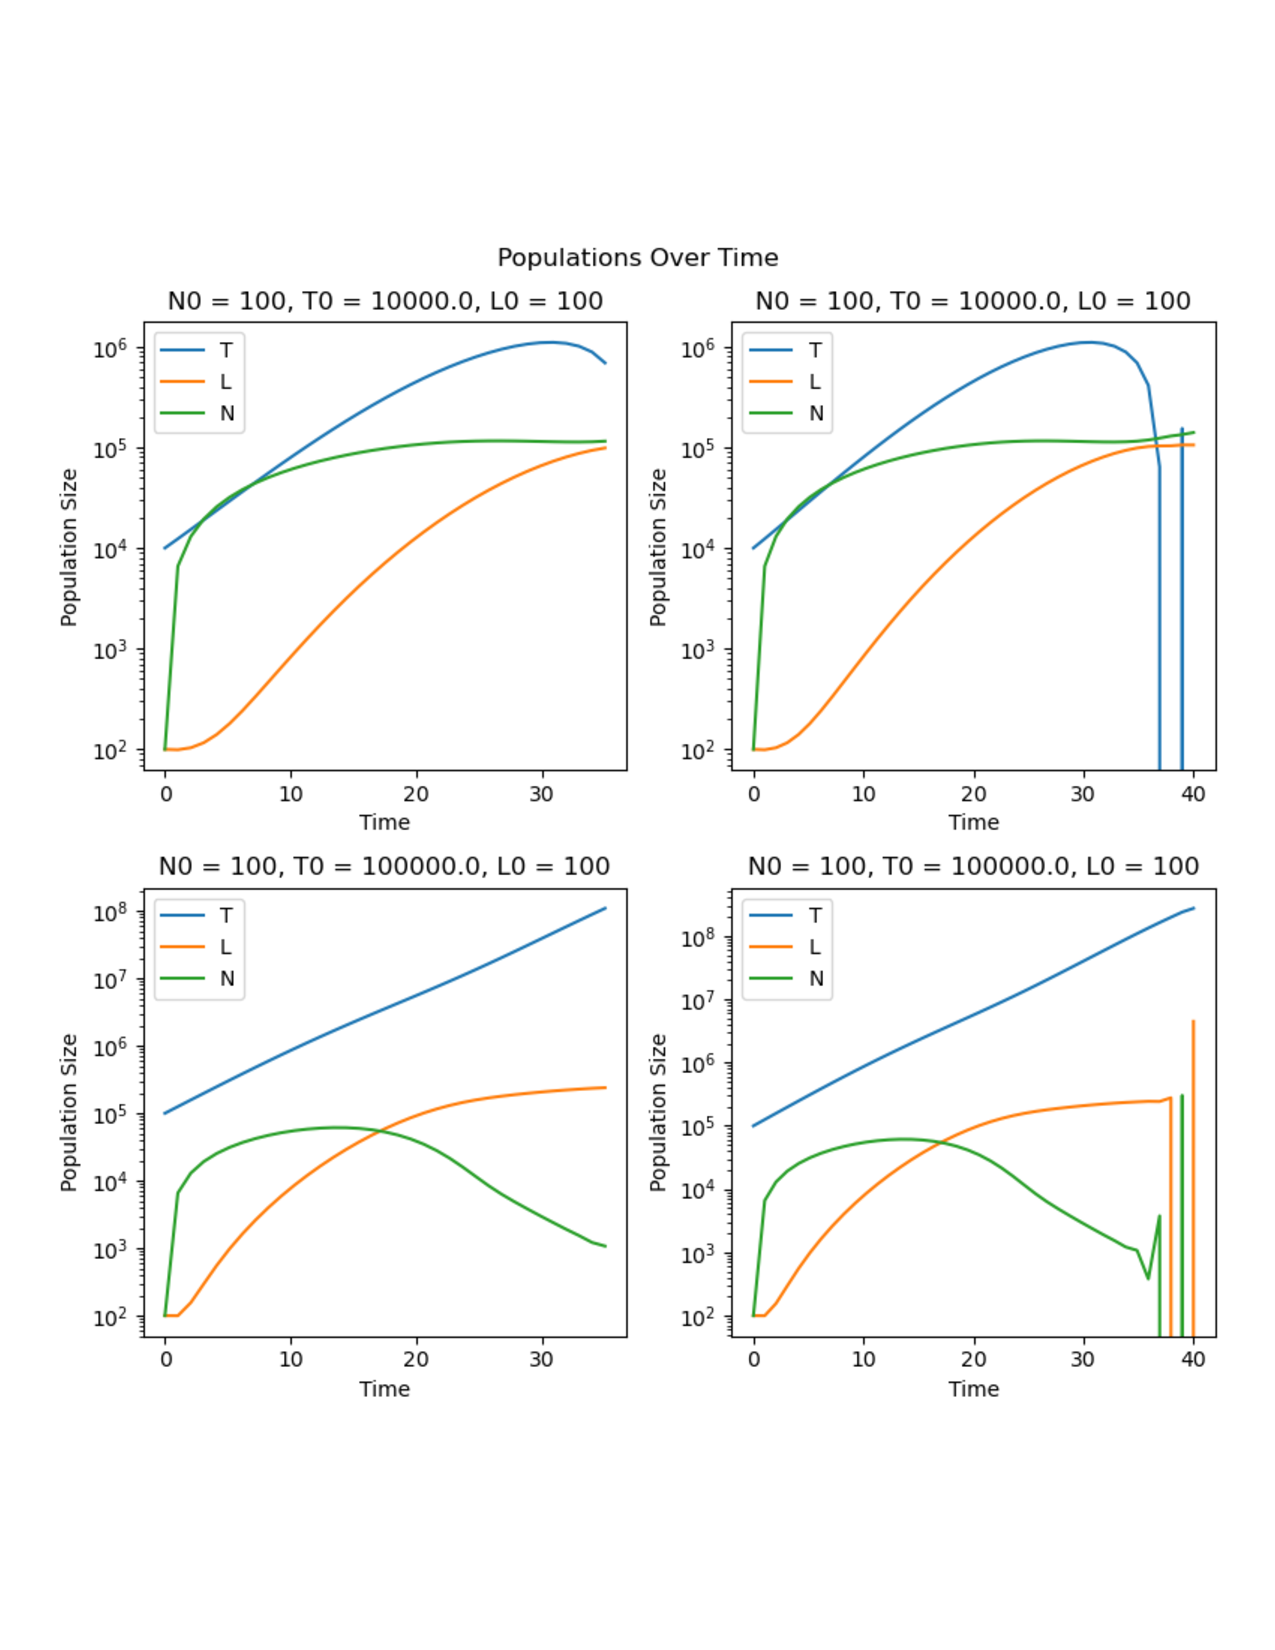
\includegraphics[scale=.6]{./images/forward_immune.pdf} % Better to make them pdfs than png or gif or jpeg
\end{center}
\caption{The Forward Euler method of each cell population generated for 2 sets of initial conditions}
\label{fig:forward} % for automatic cross referencing
\end{figure}

%%%%%%%%%%%%%%%%%%%%% Definitions %%%%%%%%%%%%%%%%%%%%%%
\section{Definitions}
\label{appendix: defs}
The following definitions are derived from the National Cancer Institute, unless otherwise stated
\begin{itemize}
	\item Adaptive Immune System: the part of the immune system that specifically targets the germs or foreign substances that are causing an infection. In order to do this, this system needs to first recognize the substance as such. Therefore, this system is slower and needs training. CB8$^+$ cells are part of this system.
	\item Cancer:  a term for diseases in which abnormal cells divide without control and can invade nearby tissues
	\item Chemotherapy: a cancer treatment where drugs are used to kill cancer cells or stop them from dividing
		\begin{itemize}
			\item Neoadjuvent Chemotherapy: chemotherapy administered before the primary treatment of the tumor is performed. Typically, surgery is the primary treatment. Its main goal is to shrink the tumor so that it is easier to remove.
			\item Adjuvent Chemotherapy: Chemotherapy administered after primary tumor treatment is administered. Its intent is to lower the risk of the cancer returning.
		\end{itemize}
	\item Cytotoxic/CD8$^+$ T-cell: is a T-lymphocyte that kills or infected cells or cells that are damaged in other ways. They are not natural killers and as such have to be trained to kill cancer. (Mayo clinic)
	\item Innate Immune System: the part of the immune system that is the first line of defense against intruders or unknown foreign cells in the body. It responds to all foreign substances in the same manner (National Library of Medicine). It can be thought of as "kill first, ask questions later." NK cells are part of this system.
	\item Log-kill Hypothesis: when growth of a cancer is exponential—increasing by a constant fraction of itself every fıxed unit of time—then in the presence of effecive anticancer drugs it also shrinks by a constant fraction \cite{LogKill}
of itself
	\item Remission: A decrease in or disappearance of signs and symptoms of cancer. In partial remission, some, but not all, signs and symptoms of cancer have disappeared. In complete remission, all signs and symptoms of cancer have disappeared, although cancer still may be in the body.
	\item Treatment cycle: the regular and repeated interval of time between each new dose of a chemotherapy drug. A cycle comprises of a rest period to allow the body to heal from the effects until the new dose is given. This information was retrieved from the American Cancer Society and\ \cite{CALEY2012186}.
	\item Tumor: an abnormal mass of tissue that forms when cells grow and divide more than they should or do not die when they should. Tumors may be \textit{benign} (not cancer) or \textit{malignant} (cancer). For this project, defined the tumor burden as the number of cancer cells in the body.
	\item Tumor burden: the size of a tumor or number of cancer cells. This is the total amount of cancer found in the body.
        \item Natural Killer Cell (NK Cell): A type of immune cell that has granules (small particles) with enzymes that can kill tumor cells or cells infected with a virus. A natural killer cell is a type of white blood cel
\end{itemize}


%%%%%%%%%%%%%%%%%%%%% Other Models and Equations%%%%%%%%%%%%%%%%%%%%%%
\section{Models}
\label{appendix: models}
In this section we give equations to models or other important terms that we discussed in our paper.

Here in is the $3\times 3$ Jacobian of our ODE system broken down by rows. 
\begin{subequations}
	\begin{equation}
		J[1] = \begin{bmatrix} k_g \ln\Bigl(\frac{T_{\max}}{T} \Bigr)  - k_g - n_{kr}N + \frac{\partial D}{\partial T} & -n_{kr} T & - \frac{\partial D}{\partial L}\end{bmatrix}\label{eq:Jrow1}
	\end{equation}
	\begin{equation}
		J[2] = \begin{bmatrix} \frac{2gTN}{h+T^2} - \frac{2gT^3 N}{(h+T^2)^2} - pN & n_D + \frac{gT^2}{h+T^2} - pT - f\mu e^{-\gamma t}& 0\end{bmatrix}\label{eq:Jrow2}
	\end{equation}
	\begin{equation}
		J[3] = \begin{bmatrix} -qL + rN - \frac{\partial}{\partial T}\Biggl( \frac{jD^2}{l_r + D^2} L \Biggr) & rT & -m+\frac{jD^2}{l_r+D^2} - \frac{2jD^3}{(l_r + D^2)^2} \frac{\partial D}{\partial L} -  f\mu e^{-\gamma t} \end{bmatrix}\label{eq:Jrow3}
	\end{equation}\label{eq:JacobianBastard}
\end{subequations}


\begin{itemize}

	\item Tumor Growth Models:
		\begin{itemize}
	\item Linear growth: 
		\begin{equation}
			\frac{\diff T}{\diff t} = k,
			\label{eq: lin}
		\end{equation}
		where $k$ is the growth rate
	\item Exponential Growth:
		\begin{equation}
			\frac{\diff T}{\diff t} = kT \label{eq: exp}
		\end{equation}
	 or with a death rate constant of $d$, $\frac{\diff T}{\diff t} = (k-d)T$
	\item Logistic Growth: 
		\begin{equation}
			\frac{\diff T}{\diff t} = kT \biggl(1- \frac{T}{T_{\max}}\biggr)\label{eq: logistic},
		\end{equation}
		where $T_{\max}$ is the max size a tumor can be, which is equivalent to the carrying capacity.
		\end{itemize}
		
	\item Chemotherapy Models: 
		\begin{itemize}
			\item Exponential Decay: Pillis and Radunskaya modeled the mix of immunotherapy and chemotherapy on tumor growth. In particular, they modeled the drug as an exponential decay given by 
				\begin{equation}
					G_M = -\gamma M \label{eq: Pillis},
				\end{equation}
				where $M=M(t)$ is the concentration of the drug in the bloodstream at some time $t$.
				
			\item Panetta also used an exponential but considering the frequency between doses as
				\begin{equation}
					g(t) = h e^{-\gamma(t-n-\tau)} \label{eq:PanettaExpDec},
				\end{equation}
				where $g(t)$ is the effects of the chemotherapy drug, $\gamma$ is the decay of the drug, $n$ is the number of doses, and $\tau$ is the period between doses.
				
			\item Personalized treatment: Ophir Nave modeled a personalizable treatment plan as 
				\begin{equation}
					\mathscr{F} = \sum_{k=0}^n q(t-mk) \mathscr{H} (t-mk)e^{\frac{t-mk}{0.5}}\label{eq: NavePersonalChemo},
				\end{equation}
				where $n$ is the duration of the treatment, $m$ is the interval between treatments, and $\mathscr{H}$ a unit step function.
		\end{itemize}
	\item Immunological Response Models:
		\begin{itemize}
			\item Pillis, Radunskaya, Wiseman:\\
                    			$\frac{dT}{dt} = aT(1-bT) - cNT - D\\$
                    			$\frac{dN}{dt} = \sigma - fN +\frac{gT^2}{h + T^2}N - pNT\\$
                    			$\frac{dL}{dt} = - mL +\frac{jD^2}{k + D^2}L - qLT + rNT\\$
                    			$D = d\frac{(L/T)^\lambda}{s + (L/T)^\lambda}T$\\
                    		Where we define each constant:
                   		 \begin{itemize}
                    			\item a = $5.14 \times 10^{-1}$ has units $\text{day}^{-1}$ is the tumor growth rate
                    			\item b = $1.02 \times 10^{-9}$ has units $\text{cell}^{-1}$ where  $\frac{1}{b}$ is the tumor carrying capacity.
                   		 	\item $N_{NR}$ = $3.23 \times 10^{-7}$ has units $\text{cell}^{-1}\text{day}^{-1}$ is the fractional cell kill(see appendix) rate of NK cells against tumors.  
                   		 	\item $sigma = 1.3 \times 10^4$ has units $\text{cells} \text{day}^{-1}$ is the constant NK cells production.
                   		 	\item $N_d = 4.12 \times 10^{-2}$ has units $\text{day}^{-1}$ is the natural death rate of NK cells.
                   		 	\item $g = 2.5 \times 10^-2$ has units $\text{day}^{-1}$ is the max NK recruitment
                   		 	\item $h = 2.02 \times 10^7$ has units $\text{cell}^2$ is the steepness coefficient of the NK recruitment curve.
                   		 	\item $p = 1.00 \times 10^{-7}$ has units $\text{cell}^{-1}\text{day}^{-1}$ is the rate at which tumors incapacitate NK cells
                   		 	\item $m = 2.00 \times 10^{-2}$ has units $\text{day}^{-1}$ is the natural death rate of CD8$^+$ cells.
                   		 	\item $j = 3.75 \times 10^{-2}$ has units $\text{day}^{-1}$ is the max CD8$^+$ recruitment rate, and the constant $k = 2 \times 10^7$ has units $\text{cell}^2$ is the steepness coefficient of the CD8+ recruitment curve.
                   		 	\item $L_R = 2 \times 10^7$ has units $\text{cell}^2$ is the steepness coefficient of the CD8$^+$ recruitment curve.
                   		 	\item $q = 3.42 \times 10^{-10}$ has units $\text{cell}^{-1}\text{day}^{-1}$ is the rate that tumors deactivate CD8$^+$ cells.
                   		 	\item $r =1.1 \times 10^{-7} $ has units $\text{cell}^{-1}\text{day}^{-1}$ is the rate at which those CD8$^+$ cells are produced. 
                    			\item $d = 5.80$ has units $\text{day}^{-1}$ is the saturation level of fractional tumor cell kill by CD8$^+$ T cells
                    			\item $s = 2.5 \times 10^{-1}$ has no units, and is the steepness of the curve which determines the Tumor vs. CD8$^+$ cell competition. Lastly, \item $\lambda = 1.36$ has no units. 
				\end{itemize}
			\item Alharbi \& Sham Rambely: their modeling equations looked at the interaction of tumor cells and the immune system, $I$, as a whole as well as normal cells , $N$, (non-immune, non-tumor cells). They described the relationships by (using a logistic growth for tumor $T$):
				\begin{eqnarray}
					\begin{aligned}
						\frac{\diff N}{\diff t} &= rN(1-\beta_1 N) - \eta NI - \gamma NT \\
						\frac{\diff T}{\diff t} &= \alpha_1T(1-\alpha_2T) + \beta_2 NT - \alpha_3 T1 \\
						\frac{\diff I}{\diff t} &= \sigma - \delta I _ \frac{\rho N I}{m+N} + \frac{\rho_1 TI}{m_1 + T} - \mu NI - \mu_1 TI \label{eq: AlharbiTumorImmuno}
					\end{aligned}
				\end{eqnarray}
			\item dePillis et. al: they modeled the primary interaction between effector cells, $E$, like CB8$^+$, and the tumor, $T$ by using logistic growth and 
				\begin{eqnarray}
					\begin{aligned}
						\frac{\diff T}{\diff t} &= a_1T(1-b_1T) - c_2ET - c_3NT - k_2(1-e^{-u}) \\
						\frac{\diff N}{\diff t} &= a_2(1-b-2N) - c_4NT - k_3 (1-e^{-u})\label{eq: dePillisTumorImmuno}
					\end{aligned}
				\end{eqnarray}
		\end{itemize}
	\item Growth-Chemo-Immune PDE System: Ansarizadeh, Singh, and Richards modeled tumor cells using a system of PDEs. Specifically, they used a logistic model for the normal cells $N$, tumor $T$, immune $I$, and the chemotherapeutic drug $U$. For them, the drug was only active for certain phases of the cell division cycle the expression $1-e^{-U}$ was used to denote the fraction of cells killed.
		\begin{eqnarray}
			\begin{aligned}
				\frac{\partial N}{\partial t} &= r_2 N (1-b_2)N - c_4TN - a_3(1-e^U)N + D_N \frac{\partial^2 N }{\partial x^2} \\
				\frac{\partial T}{\partial t} &= r_1 N (1-b_1 T) - c_2 IT - c_3TN - a_2(1-e^{-U})T + D_T \frac{\partial^2 T }{\partial x^2} \\
				\frac{\partial I}{\partial t} &= s + \frac{\rho IT}{\alpha + T} - c_1 IT - d_1 I - a_1(1-e^{-U})I +D_I \frac{\partial^2 I }{\partial x^2} \\
				\frac{\partial U}{\partial t} &= v(t) -d_2U + D_U \frac{\partial^2 U}{\partial x^2}\label{eq:GrowthChemoImmunoPDE}
			\end{aligned}
		\end{eqnarray}
\end{itemize}


%%%%%%%%%%%%%%%%%%%%%%%%%%%%%%%%%%%%%
%% Bibliography below
%%%%%%%%%%%%%%%%%%%%%%%%%%%%%%%%%%%%%
%\FloatBarrier % Keep the figures from being put after the bibliography
\newpage
%% If using bibtex, leave this uncommented
\bibliography{refs.bib} %if using bibtex, call your bibtex file refs.bib
\bibliographystyle{alpha}
\nocite{*}
%% If not using bibtex, comment out the previous two lines and uncomment those below
%\begin{thebibliography}{99}
%\bibitem{Vandermeersch} First reference goes here
%\end{thebibliography}
\end{document}
